% begin module differentiable-counterexamples
\begin{frame}
\frametitle{How Can a Function Fail to be Differentiable?}
\begin{columns}[c]
\column{.3\textwidth}
\ 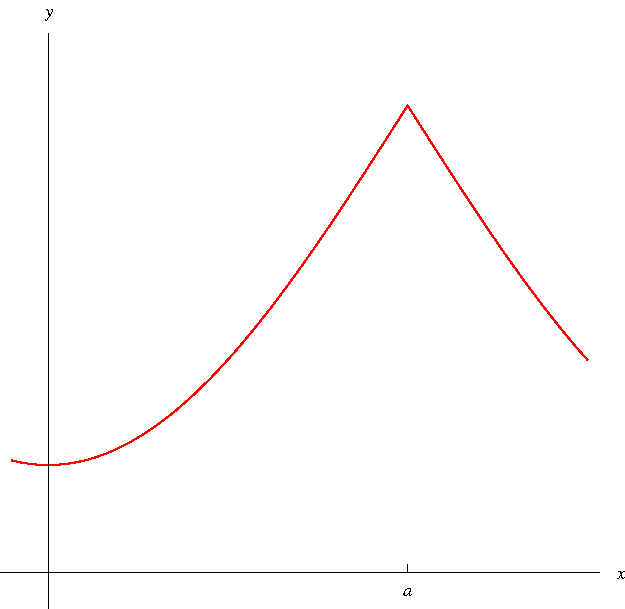
\includegraphics[height=3cm]{derivatives/pictures/03-02-noprimea.pdf}%

\uncover<2->{%
corner
}%
\column{.3\textwidth}
\ 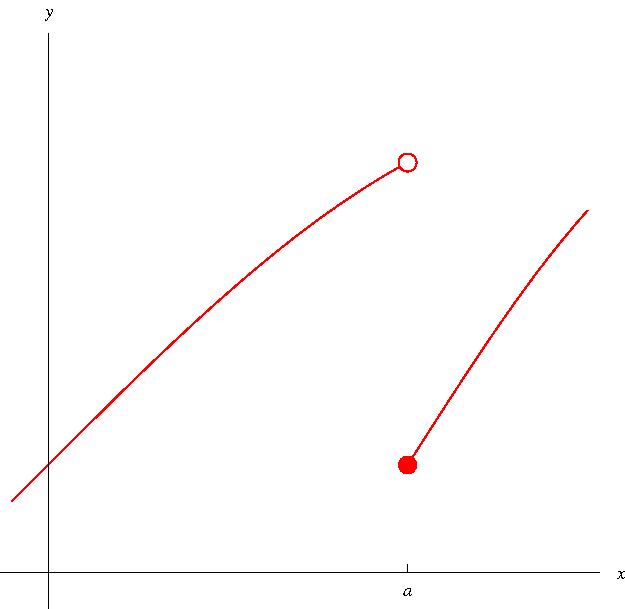
\includegraphics[height=3cm]{derivatives/pictures/03-02-noprimeb.pdf}%

\uncover<3->{%
discontinuity 
}%
\column{.3\textwidth}
\ \only<handout:0| -3>{%
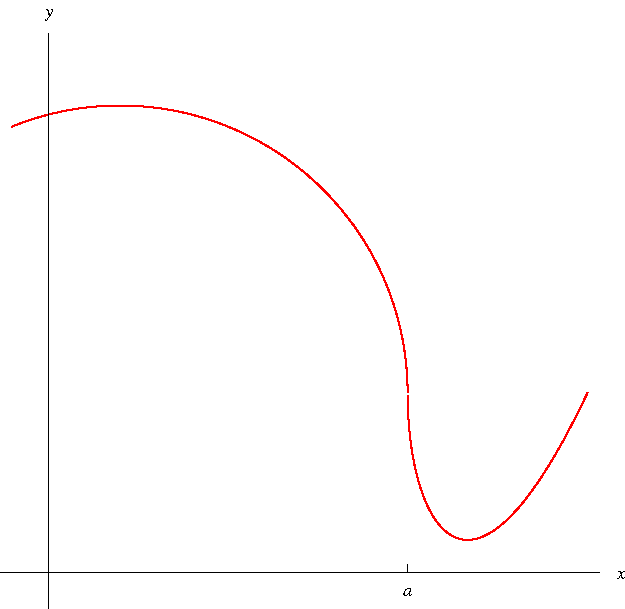
\includegraphics[height=3cm]{derivatives/pictures/03-02-noprimec.pdf}%
}%
\only<4->{%
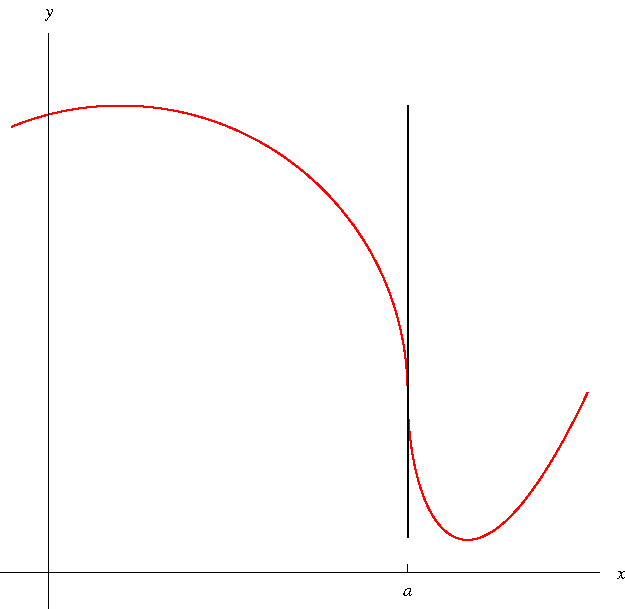
\includegraphics[height=3cm]{derivatives/pictures/03-02-noprimed.pdf}%
}%

\uncover<4->{%
vertical tangent 
}%
\end{columns}
\end{frame}
% end module differentiable-counterexamples
